% !Mode::"TeX:Utf-8"
\documentclass[winfonts,UTF8]{article}
%\documentclass[UTF8]{article}
\usepackage{amssymb}
%\usepackage{ctex}
\usepackage{amsmath}
\usepackage{listings}
\usepackage{graphicx}
%\usepackage[demo]{graphicx}

\usepackage{caption}
\usepackage{subcaption}

%\usepackage{subfig}
%\usepackage{subfigure}

\usepackage{algorithm}
\usepackage{algorithmic}
%\usepackage{epsfig,subfigure,epstopdf}
%\usepackage{tikz}

%\usepackage{CJK}

%\usepackage[pdftex]{hyperref}

\usepackage[colorlinks,linkcolor=red,anchorcolor=blue,citecolor=green]{hyperref}

\usepackage[top=1in, bottom=1in, left=1in, right=1in]{geometry}


\begin{document}

    \title{CS388 Natural Language Processing\\Homework 2: Part-of-Speech Tagging with HMMs and CRFs}
    %\centerline{\textbf{Homework 2: Part-of-Speech Tagging with HMMs and CRFs}}
    \author{Jianyu Huang}
    \maketitle

    
\section{Introduction}
We would like to explore the performance of Hidden Markov Models (HMMs) and Conditional Random Fields (CRFs) on the Part-of-Speech (POS) tagging task, based on some real-world data from the Penn Treebank\cite{laa}. I adopt the implementation of HMM and CRF from the Mallet (Machine Learning for LanguagE Toolkit) package\cite{mallet} as our code base.\\
The evaluation part in Mallet provides the overall training and testing accuracy after sequence labeling with HMM/CRF. Beyond that, I change the training and testing code in Mallet to also measure accuracy specifically for out-of-vocabulary items (OOV) \cite{laa}.\\
Finally, I compare the performance of CRF model on the data with extra orthographic features, including capitalizations, hyphens, common English suffixes, etc.

\section{Implementation}
\begin{enumerate}

\item In the first step I covert the raw data from the Penn Treebank format to the Mallet format. I modify the “POSTaggerFile.java” in the first assignment to do the preprocessing by splitting all valid tokens and replacing every backslash with a space.

\item To measure accuracy specifically for out-of-vocabulary (OOV) items, I record the number of all seen training instances in “TokenAccuracyEvaluator” class with HashSet during the first training iteration and reference it during the testing iterations. To be specific, the method “evaluateInstanceList” is modified to count the total number of OOV items in training phase and the number of correct OOV items in testing phase.

\item To add extra orthographic features to the CRF model, I implement “POSextraFeatures.java” to detect seven most common features in the preprocessing stage. The features I added are list in Table \ref{tab:orth}. (Noun suffixes, verb suffixes and adjective suffixes are from \cite{grammar})


\begin{table}[!htbp]
\centering
{\footnotesize
\begin{tabular}{l|c}
\hline
Label & Feature \\ 
\hline
\hline
gerund & end with $'$ing$'$ \\ 
\hline 
plural & end with $'$s$'$ \\ 
\hline 
hythen & contains $'$-$'$ \\ 
\hline 
caps & start with upper case characters \\ 
\hline 
noun & \begin{tabular}[x]{@{}c@{}}end with $'$-acy, -al, -ance, -ence, -dom, -er, -or, -ism,\\ 
-ist, -ity, -ty, -ment, -ness, -ship, -sion, -tion$'$\end{tabular} \\ 
\hline 
verb & end with $'$-ate, -en, -ify, -fy, -ize, -ise$'$ \\ 
\hline 
adj & end with $'$-able, -ible, -al, -esque, -ful, -ic, -ical, -ious, -ous, -ish, -ive, -less, -y$'$ \\ 
\hline 
\end{tabular} 
}
\caption{Extra Orthographic features in CRF modeling}
\label{tab:orth}
\end{table}

\item Two datasets are used for the experiment. In the small corpus \emph{atis}, we train on 80\% of the data and test on the remaining 20\%, and we average the results over 10 random training/test splits. In the large corpus \emph{wsj}, we use section 00 for training and section 01 for testing.
\end{enumerate}

\section{Experiment}
\begin{enumerate}
\item
The results for HMM, CRF using only tokens and CRF with extra orthogonal features on \emph{atis} and \emph{atis} corpora are shown in Table~\ref{tab:res} and Figure~\ref{fig:res}.

\begin{table}[!htbp]
\centering
{
\begin{tabular}{c|c|c|c|c|c|c}
\hline 
 & \multicolumn{2}{|c|}{HMM} &  \multicolumn{2}{|c|}{CRF} & \multicolumn{2}{|c}{CRF with extra features} \\ 
 \cline{2-7}
 & atis & wsj & atis & wsj & atis & wsj \\ 
\hline 
Training accuracy (\%) & 88.85\% & 86.18\% & 99.88\% & 98.36\% & 99.88\% & 99.19\% \\ 
\hline 
Testing accuracy (\%) & 86.59\% & 78.54\% & 92.62\% & 79.16\% & 94.00\% & 86.93\% \\
\hline 
OOV percentage (\%) & 2.94\% & 15.31\% & 2.94\% & 15.33\% & 2.94\% & 15.33\% \\
\hline
Testing OOV accuracy (\%) & 22.41\% & 38.03\% & 26.77\% & 46.53\% & 47.51\% & 73.30\%\\
\hline
Running time(s) & 5.239 & 78 & 94.701 & 7740 & 92.405 & 6584\\
\hline 
\end{tabular} 
}
\caption{Results of HMM, CRF using only tokens and CRF with extra orthogonal features}
\label{tab:res}
\end{table}


\begin{figure}[h]
\centering
\begin{subfigure}[b]{0.45\textwidth}
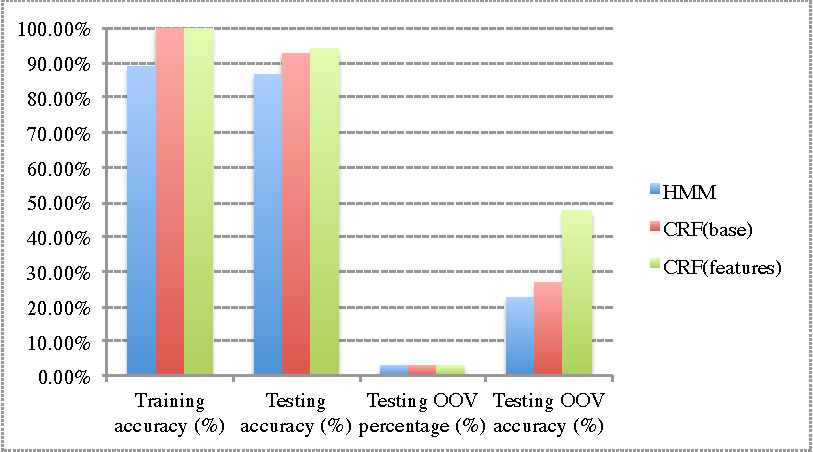
\includegraphics[width=\textwidth]{res1.pdf}
\caption{atis}
\label{fig:res_atis}
\end{subfigure}
~
\begin{subfigure}[b]{0.45\textwidth}
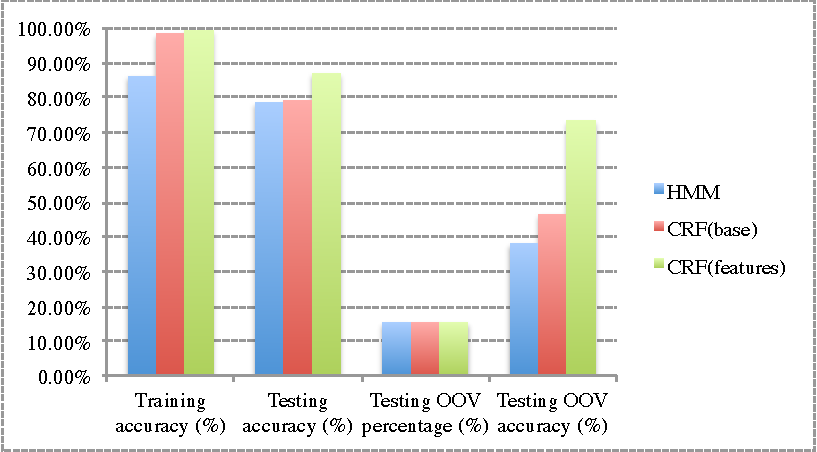
\includegraphics[width=\textwidth]{res2.pdf}
\caption{wsj}
\label{fig:res_wsj}
\end{subfigure}
\caption{Results of HMM, CRF(base) and CRF(features) on \emph{atis} and \emph{wsj} dataset}
\label{fig:res}
\end{figure}



\item
The results for adding extra orthographic features to the data are shown in Table~\ref{tab:feature} and Figure~\ref{fig:feature}.\\
\begin{table}[!htbp]
\centering 
{\footnotesize
\begin{tabular}{c|c|c|c|c|c|c|c|c|c|c}
\hline
\multicolumn{2}{c|}{}& raw & gerund & caps & plural & hyphen & noun & verb & adj & All \\
\hline
\hline
& Training accuracy (\%) & 99.88\% & 99.83\% & 99.83\% & 99.83\% & 99.83\% & 99.83\% & 99.83\% & 99.83\% & 99.88\% \\
\cline{2-11}
& Testing accuracy (\%) & 92.62\% & 93.11\% & 92.99\% & 93.57\% & 92.99\% & 93.22\% & 93.11\% & 92.99\% & 94.00\% \\
\cline{2-11}
atis& OOV percentage (\%) & 2.94\% & 2.80\% & 2.80\% & 2.80\% & 2.80\% & 2.80\% & 2.80\% & 2.80\% & 2.94\% \\
\cline{2-11}
& Testing OOV accuracy (\%) & 26.77\% & 37.50\% & 37.50\% & 41.67\% & 33.33\% & 45.83\% & 37.50\% & 33.33\% & 47.51\% \\
\cline{2-11}
& Running time(s) & 94.7008 & 97.78 & 93.867 & 99.918 & 101.494 & 101.79 & 100.146 & 87.959 & 92.4047 \\
\hline
\hline
& Training accuracy (\%) & 98.36\% & 98.61\% & 99.14\% & 98.35\% & 98.61\% & 98.63\% & 98.62\% & 98.62\% & 99.19\% \\
\cline{2-11}
& Testing accuracy (\%) & 79.16\% & 80.44\% & 82.57\% & 81.93\% & 79.98\% & 80.20\% & 79.66\% & 79.84\% & 86.93\% \\
\cline{2-11}
wsj& OOV percentage (\%) & 15.33\% & 15.33\% & 15.33\% & 15.33\% & 15.33\% & 15.33\% & 15.33\% & 15.33\% & 15.33\% \\
\cline{2-11}
& Testing OOV accuracy (\%) & 46.53\% & 50.76\% & 56.36\% & 57.77\% & 48.89\% & 50.06\% & 47.66\% & 47.94\% & 73.30\% \\
\cline{2-11}
& Running time(s) & 7740 & 8202 & 12390 & 7645 & 8044 & 6499 & 6876 & 7394 & 6584 \\
\hline

\end{tabular} 
}
\caption{Results of adding extra orthogonal features to CRF}
\label{tab:feature}
\end{table}


\begin{figure}[!htbp]
\centering
\addtocounter{subfigure}{-2}
\begin{subfigure}[]{0.8\textwidth}
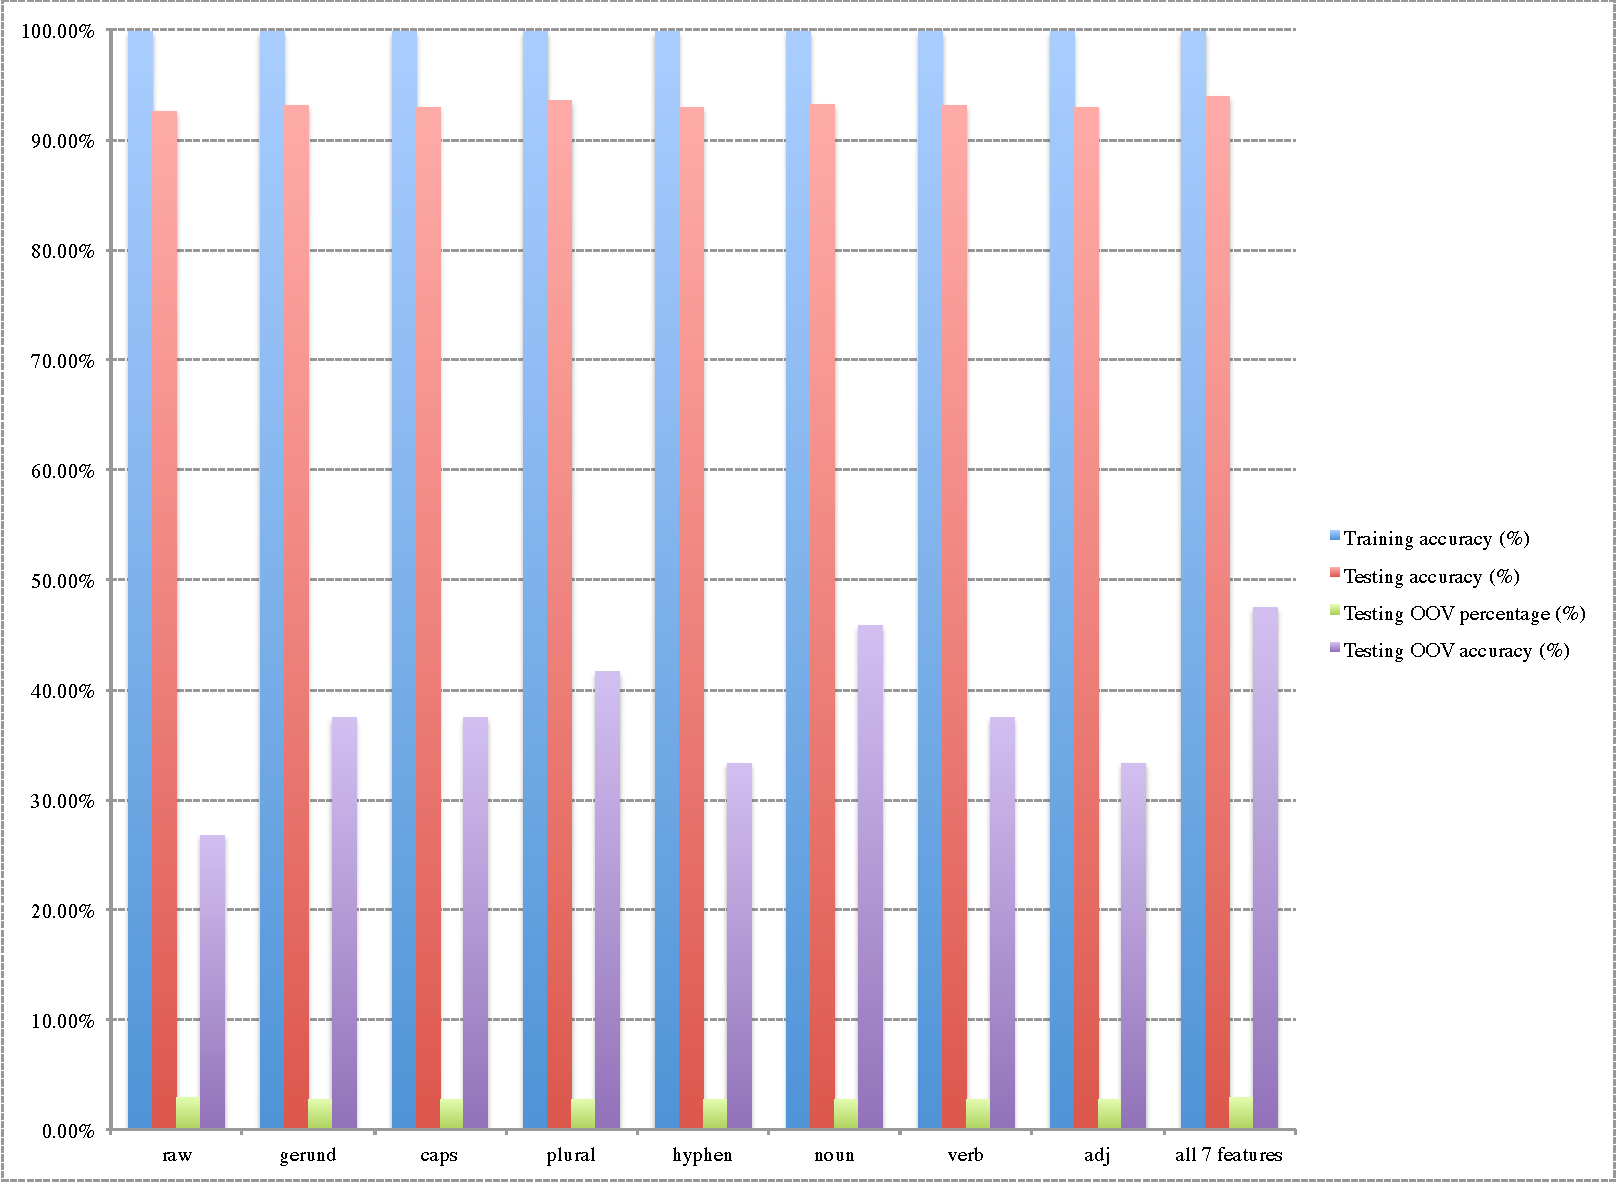
\includegraphics[width=\textwidth]{res3.pdf}
\caption{atis}
\label{fig:feature_atis}
\end{subfigure}
~
\begin{subfigure}[]{0.8\textwidth}
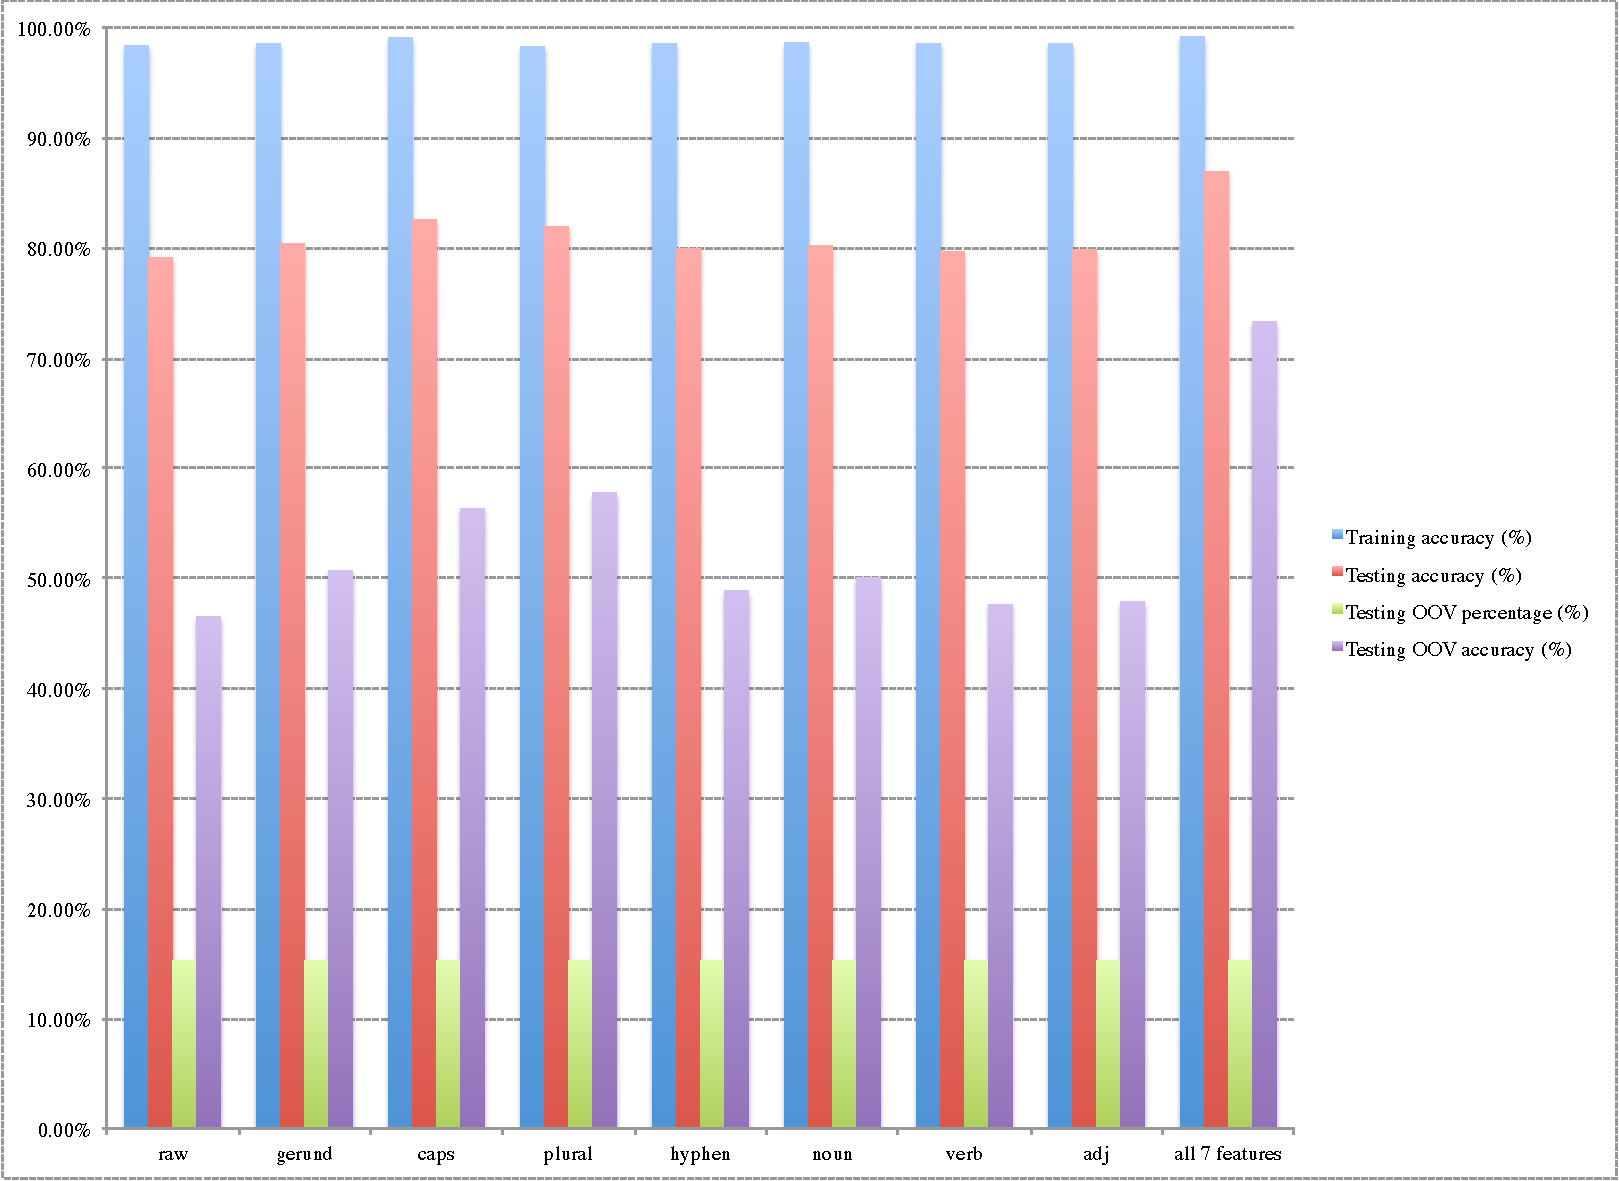
\includegraphics[width=\textwidth]{res4.pdf}
\caption{wsj}
\label{fig:feature_wsj}
\end{subfigure}
\caption{Results of adding extra orthogonal features to CRF model on \emph{atis} and \emph{wsj} dataset}
\label{fig:feature}
\end{figure}

\item
In addition to the basic experiment, I also finish some extension experiments, which is included in the Appendix section.

\end{enumerate}


\section{Discussion}
\subsection{Comparison between HMM and CRF}
\begin{enumerate}
\item For both dataset, the training accuracy, the overall testing accuracy, the OOV testing of CRF are all greater than those of HMM. There are several reasons: \\
\begin{itemize}
\item The discriminative models are more accurate than generative models at sequence labeling.
\item CRF is modeled by maximizing conditional likelihood $p(y|x)$ while HMM is simply trained by maximizing likelihood of data $p(x, y)$.
\item The feature dependency is considered by feature weighs in CRF, while the features are assumed independent in HMM.
\end{itemize}

\item For both dataset, the run time of CRF is much longer than that of HMM (roughly 20x for \emph{atis}, and 80x for \emph{wsj}).
\begin{itemize}
\item In each iteration CRF takes more time than HMM
\begin{itemize}
\item CRF models the dependencies between each state, so the optimization procedure in each iteration will take more time.
\item The sequence tagging results are inference of both training and testing corpora in each iteration in CRF, while that is done only after convergence in HMM.
\end{itemize}
\item CRF takes more iterations to converge than HMM.
\begin{itemize}
\item The convergence speed in CRF is slower than HMM.
\end{itemize}

\end{itemize}

\end{enumerate}
\subsection{Analysis of Adding Orthographic Features}
\begin{enumerate}
\item For both dataset, adding orthographic features increase the accuracy (both overall and OOV) and decrease running time.
\begin{itemize}
\item Orthographic features provide valuable information on OOV words for sequence tagging so that the accuracy is increased.
\item Orthographic features provide additional information to help the optimization converge faster so that the iteration times decreased. Thus finally the run time is decreased.
\end{itemize}
\item From the comparison in Figure~\ref{fig:feature}, we can see that \emph{noun} is the most useful feature for improving the performance on \emph{atis} dataset, while \emph{plural} feature helps the most important feature on \emph{wsj} dataset.

\end{enumerate}


\section{Conclusion}
Through this assignment, We explore the performance of Hidden Markov Models (HMMs) and Conditional Random Fields (CRFs) on the Part-of-Speech (POS) tagging task. It turns out that CRF is more accurate than HMM for POS tagging, but cost more time.





%

\section{Apendix} \label{appendix}

\subsection{Extension Experiments}

\begin{enumerate}
\item Larger data set experiment\\
I train on section 02, 03 and test on section 04, 05 for \emph{wsj} dataset.\\
\textbf{Observation}: with larger training set, the result is more accurate. Still, CRF with extra orthogonal features has the best performance.

\item HMM on \emph{wsj} with even larger datasets\\
I test HMM over even larger data set (the $x$-$axis$ represents how many sections I use to train and test).\\
\textbf{Observation}: accuracy increases and OOV percentage decreases over larger data.

\item Change the number of iteration\\
I sample the interation number for the first extension experiment, CRF using only tokens over \emph{wsj} dataset (the $x$-$axis$ indicates the number of iterations).\\
\textbf{Observation}: more iteration means more accuracy and the improvement in early iterations is larger than that in later iterations.

\begin{figure}[h]
%\centering
\begin{subfigure}[b]{0.45\textwidth}
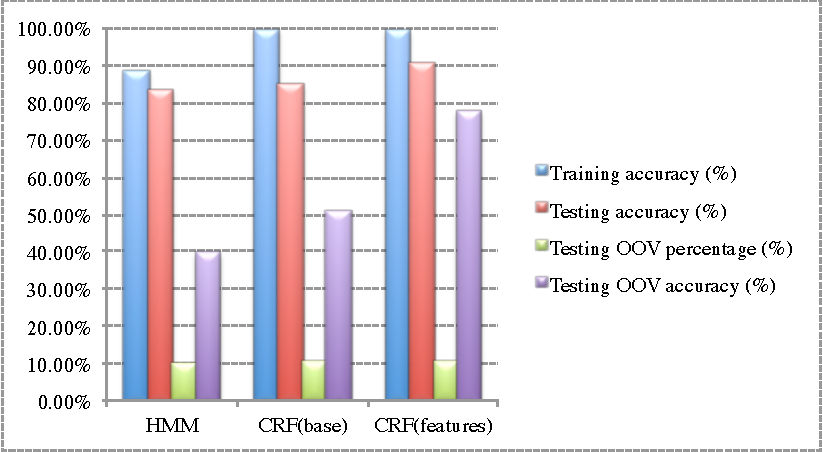
\includegraphics[width=\textwidth]{res5.pdf}
\caption{Larger data set experiment}
\label{fig:res_ext1}
\end{subfigure}
~
\begin{subfigure}[b]{0.45\textwidth}
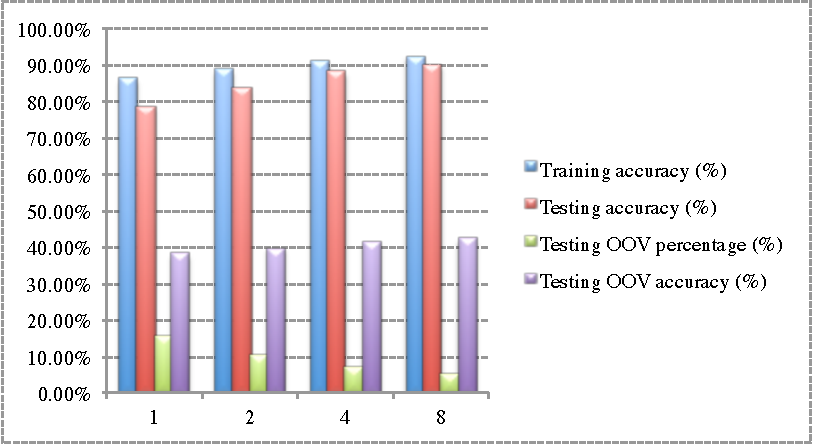
\includegraphics[width=\textwidth]{res6.pdf}
\caption{HMM on \emph{wsj} with even larger datasets}
\label{fig:res_ext2}
\end{subfigure}
~
\begin{subfigure}[b]{0.45\textwidth}
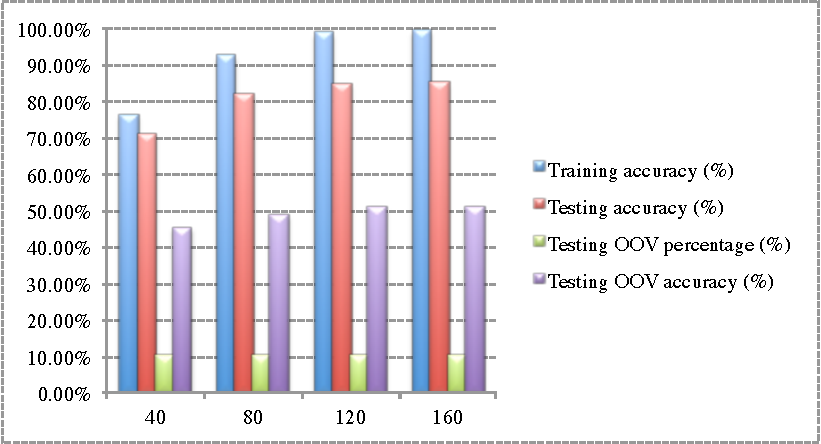
\includegraphics[width=\textwidth]{res7.pdf}
\caption{Change the number of iteration}
\label{fig:res_ext3}
\end{subfigure}


\caption{Extension Experiments}
\label{fig:res}
\end{figure}


%\begin{table}[h]
%\centering
%{
%\begin{tabular}{|c|c|c|c|}
%\hline
% & HMM & CRF(base) & CRF(features)\\
%\hline
%Training accuracy (\%) & 88.33\% & 99.44\% & 99.31\%\\
%\hline
%Testing accuracy (\%) & 83.39\% & 84.86\% & 90.31\%\\
%\hline
%Testing OOV percentage (\%) & 10.33\% & 10.34\% & 10.34\%\\
%\hline
%Testing OOV accuracy (\%) & 39.58\% & 50.94\% & 77.76\%\\
%\hline
%Running time(s) & 372 & 58752 & 53916\\
%\hline
%\end{tabular} 
%}
%\end{table}

\subsection{Testing result}
Two datasets are used for the experiment. In the small corpus \emph{atis}, we train on 80\% of the data and test on the remaining 20\%, and we average the results over 10 random training/test splits. In the large corpus \emph{wsj}, we use section 00 for training and section 01 for testing. All the results are stored in "hw2.xlsx" file.



\end{enumerate}



\section{Reference}
\renewcommand\refname{\vskip -0.25cm}
\refname
\bibliographystyle{plain}
\bibliography{hw2}



\end{document} 
















